

\documentclass[letterpaper, 11pt]{article}



\usepackage[margin=1in]{geometry}
\usepackage{setspace}\onehalfspace
\usepackage{microtype}


\usepackage{amsmath} \allowdisplaybreaks
\usepackage{amssymb}
\usepackage{amsthm} \theoremstyle{definition}
\newtheorem{theorem}{Theorem}
\newtheorem{lemma}{Lemma}
\newtheorem{assumption}{Assumption}
\newtheorem{proposition}{Proposition}
\newtheorem{definition}{Definition}


\usepackage{natbib}
\usepackage{bibentry}


\usepackage{booktabs}
\usepackage{graphicx}
\usepackage{appendix}
\usepackage[counterclockwise]{rotating} % for sidewaystable
\usepackage{subcaption}

\usepackage{url}
\usepackage[bookmarks=false,hidelinks]{hyperref}


%\usepackage{authblk}
%\renewcommand\Authfont{\sf\Large}
%\renewcommand\Affilfont{\rm\small}





%%%%%%%%%%%%%% MACRO %%%%%%%%%%%%%%%%%%%%%%%%%%%%%%%%%%%%%%
\newcommand{\email}[1]{{\href{mailto:#1}{\nolinkurl{#1}}}}

\usepackage{bm}
\renewcommand{\vec}[1]{\bm{#1}}
\newcommand{\mat}[1]{\bm{#1}}

\usepackage{xcolor}
\newcommand{\note}[1]{{\Large\bf#1}}
\newcommand{\bluenote}[1]{{\Large\color{blue}#1}}
\newcommand{\rednote}[1]{{\Large\color{red}#1}}

\usepackage{etoolbox}
% To use, for example, \Ac for \mathcal{A}.  Requires "etoolbox" package
\makeatletter
\def\do#1{\@namedef{#1c}{\ensuremath{\mathcal{#1}}}}
\docsvlist{A,B,C,D,E,F,G,H,I,J,K,L,M,N,O,P,Q,R,S,T,U,V,W,X,Y,Z}
\makeatother

\def\Eb{\mathbb{E}}
\def\Rb{\mathbb{R}}
%\def\response{[$\Longrightarrow$]}

\newenvironment{response}
{ [$\Longrightarrow$]\sf }
{ \hfill \rule{1ex}{1ex} }

\newcommand{\dx}{\mathop{}\!\mathrm{d}x}
\newcommand{\dy}{\mathop{}\!\mathrm{d}y}
\newcommand{\dz}{\mathop{}\!\mathrm{d}z}
\newcommand{\dt}{\mathop{}\!\mathrm{d}t}

\renewcommand{\bar}[1]{\mkern 1.5mu\overline{\mkern-1.5mu#1\mkern-1.5mu}\mkern 1.5mu}

%%%%%%%%%%%%%%%%%%%%%%%%%%%%%%%%%%%%%%%%%%%%%%%%%%%%%%%%



\title{A LaTeX Template for Writing Papers}
\author{Author Name \and Another Name \and Changhyun Kwon\footnote{Corresponding Author: \email{chkwon@buffalo.edu}}}
\date{Department of Industrial and Systems Engineering\\University at Buffalo\\[0.5cm] February 16, 2015}

%\usepackage{showlabels} 
%\usepackage[final]{showlabels}


\begin{document}
\maketitle

\begin{abstract}
This document provides some useful tips as well as serve a template for writing a paper in LaTeX. To understand how LaTeX works, you should compare the source code and the output PDF.\\
\noindent\textbf{Keywords:} keyword1; keyword2; keyword3
\end{abstract}



\section{Test} \label{sec:paragraph}
In LaTeX, just enter an empty line for a new paragraph.

Like this. blah blah blah blah blah blah blah blah blah blah blah blah blah blah blah blah blah blah blah blah blah blah blah blah blah blah blah blah blah blah blah blah blah blah blah blah blah blah blah blah blah blah blah blah blah blah blah blah.

Don't use double backslashed to change a line. Backslashed will be used in tables and equations only. Some random text here, there, and everywhere. Some random text here, there, and everywhere. Some random text here, there, and everywhere. Some random text here, there, and everywhere. Some random text here, there, and everywhere.  \\
If you use double backslashes to change a line, it will look very bad. Some random text here, there, and everywhere. Some random text here, there, and everywhere. Some random text here, there, and everywhere. Some random text here, there, and everywhere. Some random text here, there, and everywhere. 

If you want to \emph{emphasize} some \emph{words}, use \emph{emph}, instead of \textit{textit}.




\section{Citation} \label{sec:citation}

\begin{itemize}
\item Textual citation: \citet{Kwon2013rsp}
\item Parenthetical citation: \citep{Kwon2013rsp}
\item Multiple parenthetical citations: \citep{Bertsimas2004,Chaerani2005,Kouvelis1996,gabrel2012recent}
\item If you need multiple \emph{textual} citations, it is better to write: \citet{Bertsimas2004}, \citet{Chaerani2005}, \citet{Kouvelis1996}, and \citet{gabrel2012recent}, instead of \citet{Bertsimas2004,Chaerani2005,Kouvelis1996,gabrel2012recent}.

\end{itemize}

See them in action:
\begin{quote}
In this paper, we propose a robust optimization framework for the routing methods based on the CVaR risk measure, assuming that data are uncertain within given sets. The proposed robust optimization method is closely related to robust shortest path (RSP) problems, which find a path that minimizes the worst-case travel cost with an uncertain set of travel cost data. When the uncertain set is box-constrained, the RSP problem can be solved in polynomial time \citep{Bertsimas2003network}, while the problem is NP-hard when the uncertain set is an ellipsoid \citep{Bertsimas2004,Chaerani2005} and a set of scenarios \citep{Kouvelis1996}. We refer readers to \citet{ben2009robust} and \citet{gabrel2012recent} and references therein for general robust optimization methods. 
\end{quote}




\section{Math} \label{sec:math}
Inline equations can be like $\sum_{j:(i,j)\in\Ac} x_{ij}$.

A single line equation:
\begin{equation}
	\sum_{j:(i,j)\in\Ac} x_{ij} = 1 \quad \forall i\in\Nc \label{node_constraint1}
\end{equation}
I used $\Ac$ as a shorthand for $\mathcal{A}$. 

Try to give some consistency in your notation. I usually use calligraphic letters to denote sets like set of nodes $\Nc$, set of arcs $\Ac$, set of shipments $\Sc$ as in $n\in\Nc$ or $\sum_{s\in\Sc} z_s$, and so on. Lower-case alphabets for variables like $x_{ij}$, $y_i$, and $z_j$. Upper-case roman alphabets like $N$, $A$, and $S$ for constants as in $n=1,...,N$ or $\sum_{s=1}^S x_s$. 

I usually use lower-case Greek letters for dual variables: $\lambda_i$, $\rho_j$, etc. Upper-case Greek letters may be some special sets or sets of dual variables: $\Lambda$, $\Theta$, etc.

Multiple lines:
\begin{align}
	\sum_{j:(i,j)\in\Ac} x_{ij} = 1 \quad & \forall i\in\Nc \label{node_constraint2} \\
	\sum_{j:(i,j)\in\Ac} y_{ij} = 1 \quad & \forall i\in\Nc \nonumber \\
	\sum_{j:(i,j)\in\Ac} z_{ij} = 1 \quad & \forall i\in\Nc \label{node_constraint3} \\
	\sum_{j:(i,j)\in\Ac} \omega_{ij} = 1 \quad & \forall i\in\Nc \label{node_constraint4} \\
	\sum_{j:(i,j)\in\Ac} \eta_{ij} = 1 \quad & \forall i\in\Nc \label{node_constraint5} 
\end{align}

A single equation that stretches to multiple lines
\begin{multline}
	\sum_{j:(i,j)\in\Ac} x_{ij} + \sum_{j:(i,j)\in\Ac} x_{ij} + \sum_{j:(i,j)\in\Ac} x_{ij} \\
	+ \sum_{j:(i,j)\in\Ac} x_{ij} +	\sum_{j:(i,j)\in\Ac} x_{ij} + \sum_{j:(i,j)\in\Ac} x_{ij} \\
	+ \sum_{j:(i,j)\in\Ac} x_{ij} +	\sum_{j:(i,j)\in\Ac} x_{ij} + \sum_{j:(i,j)\in\Ac} x_{ij} \\
	+ \sum_{j:(i,j)\in\Ac} x_{ij} + \sum_{j:(i,j)\in\Ac} x_{ij} = 1 
\end{multline}

When you want cross-referencing, do this: \eqref{node_constraint1}, or \eqref{node_constraint2}--\eqref{node_constraint5}.

If you don't want numbering, just add *, like:
\begin{equation*}
	\sum_{j:(i,j)\in\Ac} x_{ij} = 1 \quad \forall i\in\Nc
\end{equation*}
or
\[
	\sum_{j:(i,j)\in\Ac} x_{ij} = 1 \quad \forall i\in\Nc
\]
or
\begin{align*}
	\sum_{j:(i,j)\in\Ac} x_{ij} = 1 \quad & \forall i\in\Nc \\
	\sum_{j:(i,j)\in\Ac} y_{ij} = 1 \quad & \forall i\in\Nc \\
\end{align*}

Please do not use words for variables. 
\begin{itemize}
\item Don't:
	\[
		counter_1 = 3 + 10 
	\]
	where $counter_1$ may be confused with $c \times o \times u \times n \times t \times e \times r_1$.

\item Instead do:
	\[
		c_i = 3 + 10
	\]
	or
	\[
		\text{counter}_1 = 3 + 10
	\]
	or
	\[
		\textsf{counter}_1 = 3 + 10
	\]
depending on the context.
\end{itemize}


You can use $\vec{x}$ as a vector of $x_{ij}$. Some matrices $\mat{A}$ and $\mat{B}$.

Some vectors are here:
\[
	\vec{y} = \begin{bmatrix} 3 \\ 2 \\ 1 \end{bmatrix}, \qquad
	\vec{z} = \begin{bmatrix} z_1 \\ z_2 \\ \vdots \\ z_n \end{bmatrix}
\]
A matrix is here:
\[
	\mat{A} = \begin{bmatrix} a_{11} & \cdots & a_{22}  \\
							  \vdots & \ddots & \vdots  \\
							  a_{1n} & \cdots & a_{nn}  \end{bmatrix}
\]
If you like curly brackets:
\[
	\mat{A} = \begin{pmatrix} a_{11} & \cdots & a_{22}  \\
							  \vdots & \ddots & \vdots  \\
							  a_{1n} & \cdots & a_{nn}  \end{pmatrix}
\]




\section{Tables}


\begin{table} \centering
\caption{The table caption is above the table. Text to the left, numbers to the right. }
\label{tbl:example}
\begin{tabular}{l l r r}
\toprule
Name		& Location		&  Number	& Number \\
\midrule
Michael		& Chicago			&      10   &   3.190  \\
Sara		& Montreal			&     110   & 123.148  \\
Sandra		& LA				&    1210   &   3.000  \\
Alexander	& San Francisco		&       8   &   0.000  \\
\bottomrule
\end{tabular}
\end{table}

\begin{table} \centering
\caption{A bad presentation.}
\label{tbl:bad_example}
\begin{tabular}{c c l l}
\toprule
Name		& Location		&  Number	& Number \\
\midrule
Michael		& Chicago			&      10   &   3.190  \\
Sara		& Montreal			&     110   & 123.148  \\
Sandra		& LA				&    1210   &   3.000  \\
Alexander	& San Francisco		&       8   &   0.000  \\
\bottomrule
\end{tabular}
\end{table}

When you prepare tables, please just ignore the positioning of tables in the final PDF file. I put the code for Table \ref{tbl:example} above this text and the code for Table \ref{table:8-node} below this text. Their actual locations in the output PDF file will be determined by LaTeX. Table \ref{tbl:bad_example} is a bad presentation of Table \ref{tbl:example}. Tables \ref{tbl:example}--\ref{table:8-node} are small tables. If you have a big table like Table \ref{table:EDOandLINGO}, then you can use `\texttt{sidewaystable}'. However, it is best to redesign the table and not to use sideway tables. Think one more time to decide if you really need such a big table to make your arguments clear. 


\begin{table}  \centering
\caption{Arc attributes for the 8-node network, with $\rho_a$: the population density along arc $a$ and $c_a(v_a)=A_a(1 + 0.15{(v_a/l_a)}^4)$.} 
\label{table:8-node}%
\begin{tabular}{rrrrr}
\toprule
\multicolumn{2}{c}{\text{Arc $a$}}   & 				&			&			\\
\cmidrule(lr){1-2}
Start & End & $A_a$ & $l_a$ & $\rho_a$ \\
\midrule
    1 &   2 &     6 &   900 &      701\\
    1 &   3 &     4 &  1400 &    11193\\
    2 &   3 &     6 &   700 &     1701\\
\bottomrule
\end{tabular}
\end{table}


\begin{sidewaystable}
\caption{A sideway table.}
\label{table:EDOandLINGO}
\begin{tabular}{r rrrr rrrr rrrr}
\toprule
& \multicolumn{4}{c}{LINGO} & \multicolumn{4}{c}{Modified EDO} & \multicolumn{4}{c}{2-Step EDO} \\
\cmidrule(lr){2-5} \cmidrule(lr){6-9} \cmidrule(lr){10-12} 
Case &     Solution &    Risk &     Toll &   Run   &    Risk &    Toll &   Run & Objective   &    Risk &    Toll &    Run & Objective \\
     &         Type &         &  Revenue &  Time   &         & Revenue &  Time &  Gap (\%)   &         & Revenue &   Time &  Gap (\%) \\
\midrule
   1 &       Global & 2469.86 &        0 & 4 sec   & 2945.94 &  703.28 & 8 sec &     47.75   & 2469.86 &    1.96 & 14 sec &      0.08 \\
\bottomrule
\end{tabular}
\end{sidewaystable}





\section{Figures} \label{sec:figures}


\begin{figure} \centering
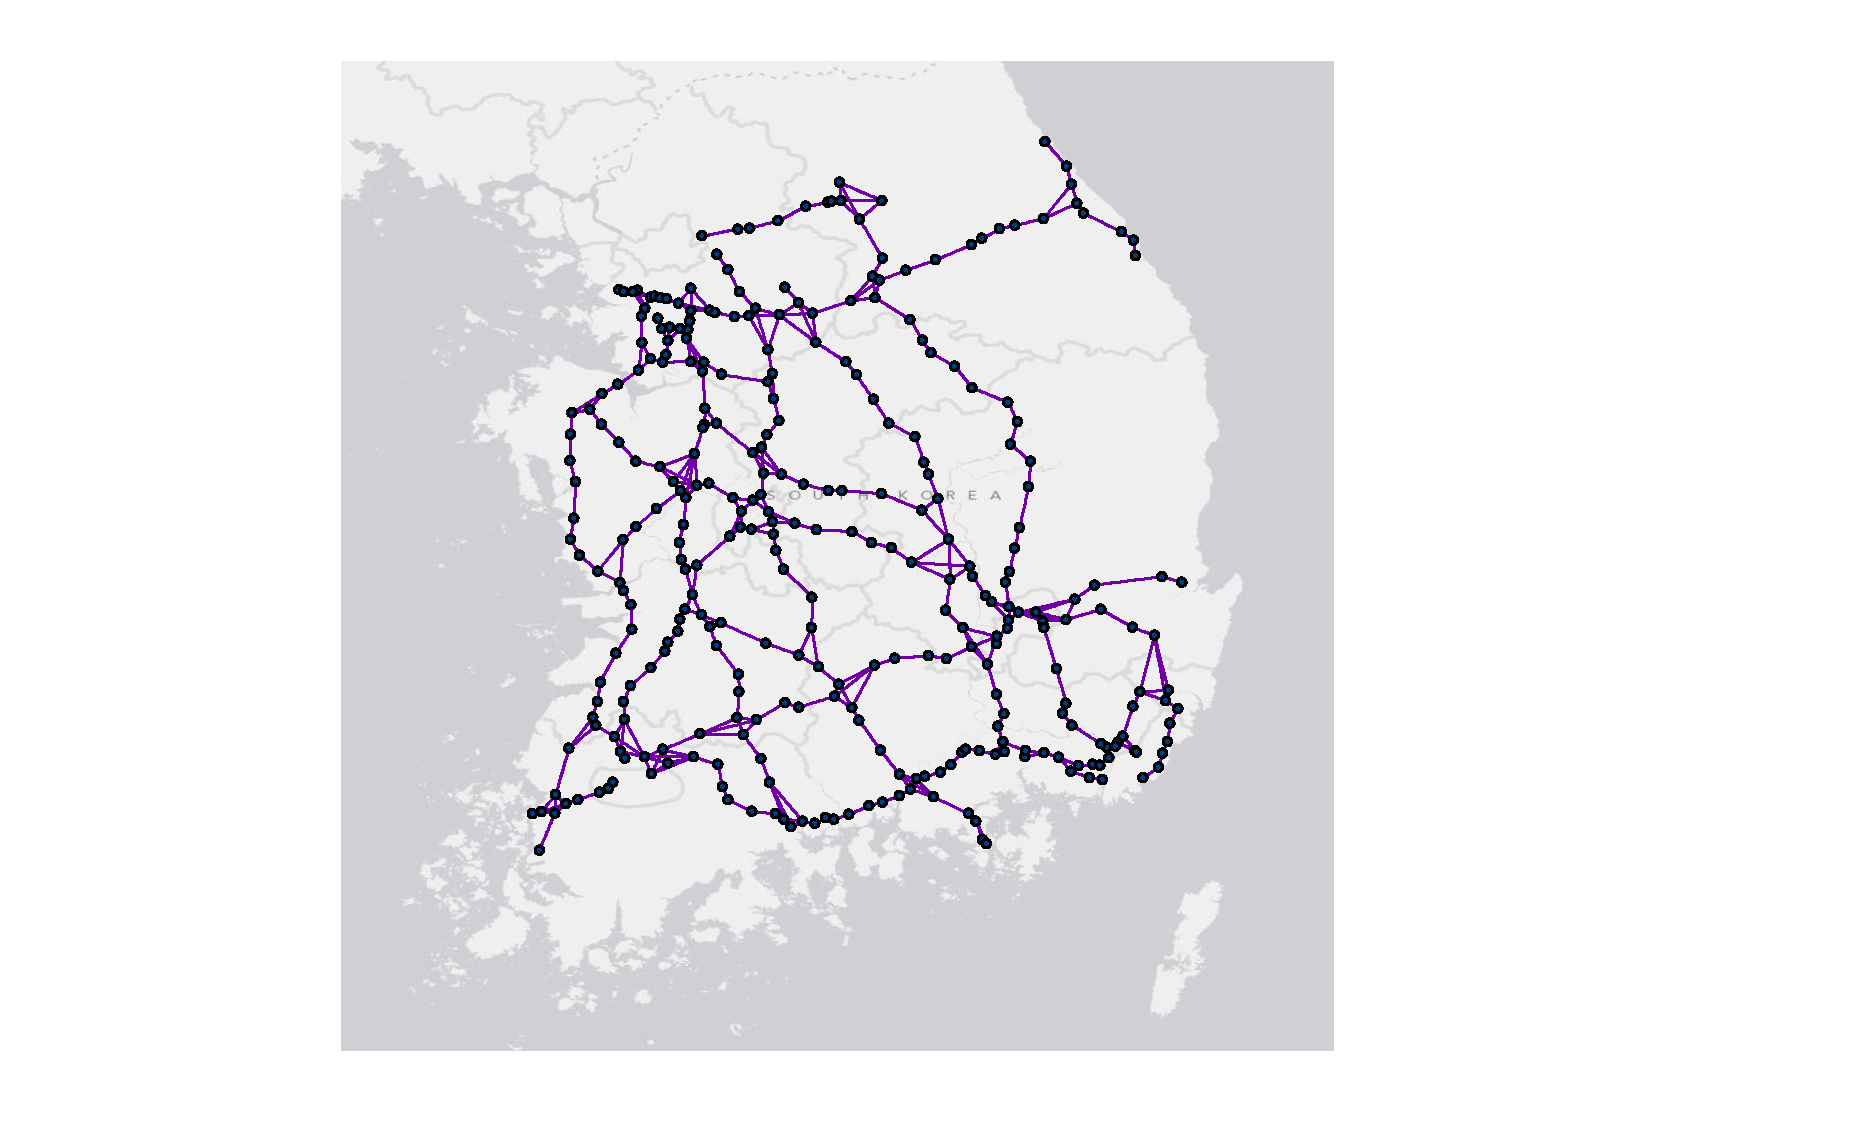
\includegraphics[width=0.45\textwidth]{map}
\caption{Figure caption is below the figure.}
\label{fig:map}
\end{figure}

For figures, it is better to put the caption below the figure. See Figure \ref{fig:map}. Whenever possible, you should save your figure as a vector-based PDF file. PDF files that were converted from a JPG file do not look good. Compare Figures \ref{fig:map-pdf} and \ref{fig:map-jpg}. As you have already seen in Figure \ref{fig:side-by-side}, you can put figures side by side.



\begin{figure} \centering
\begin{subfigure}[b]{0.4\textwidth}
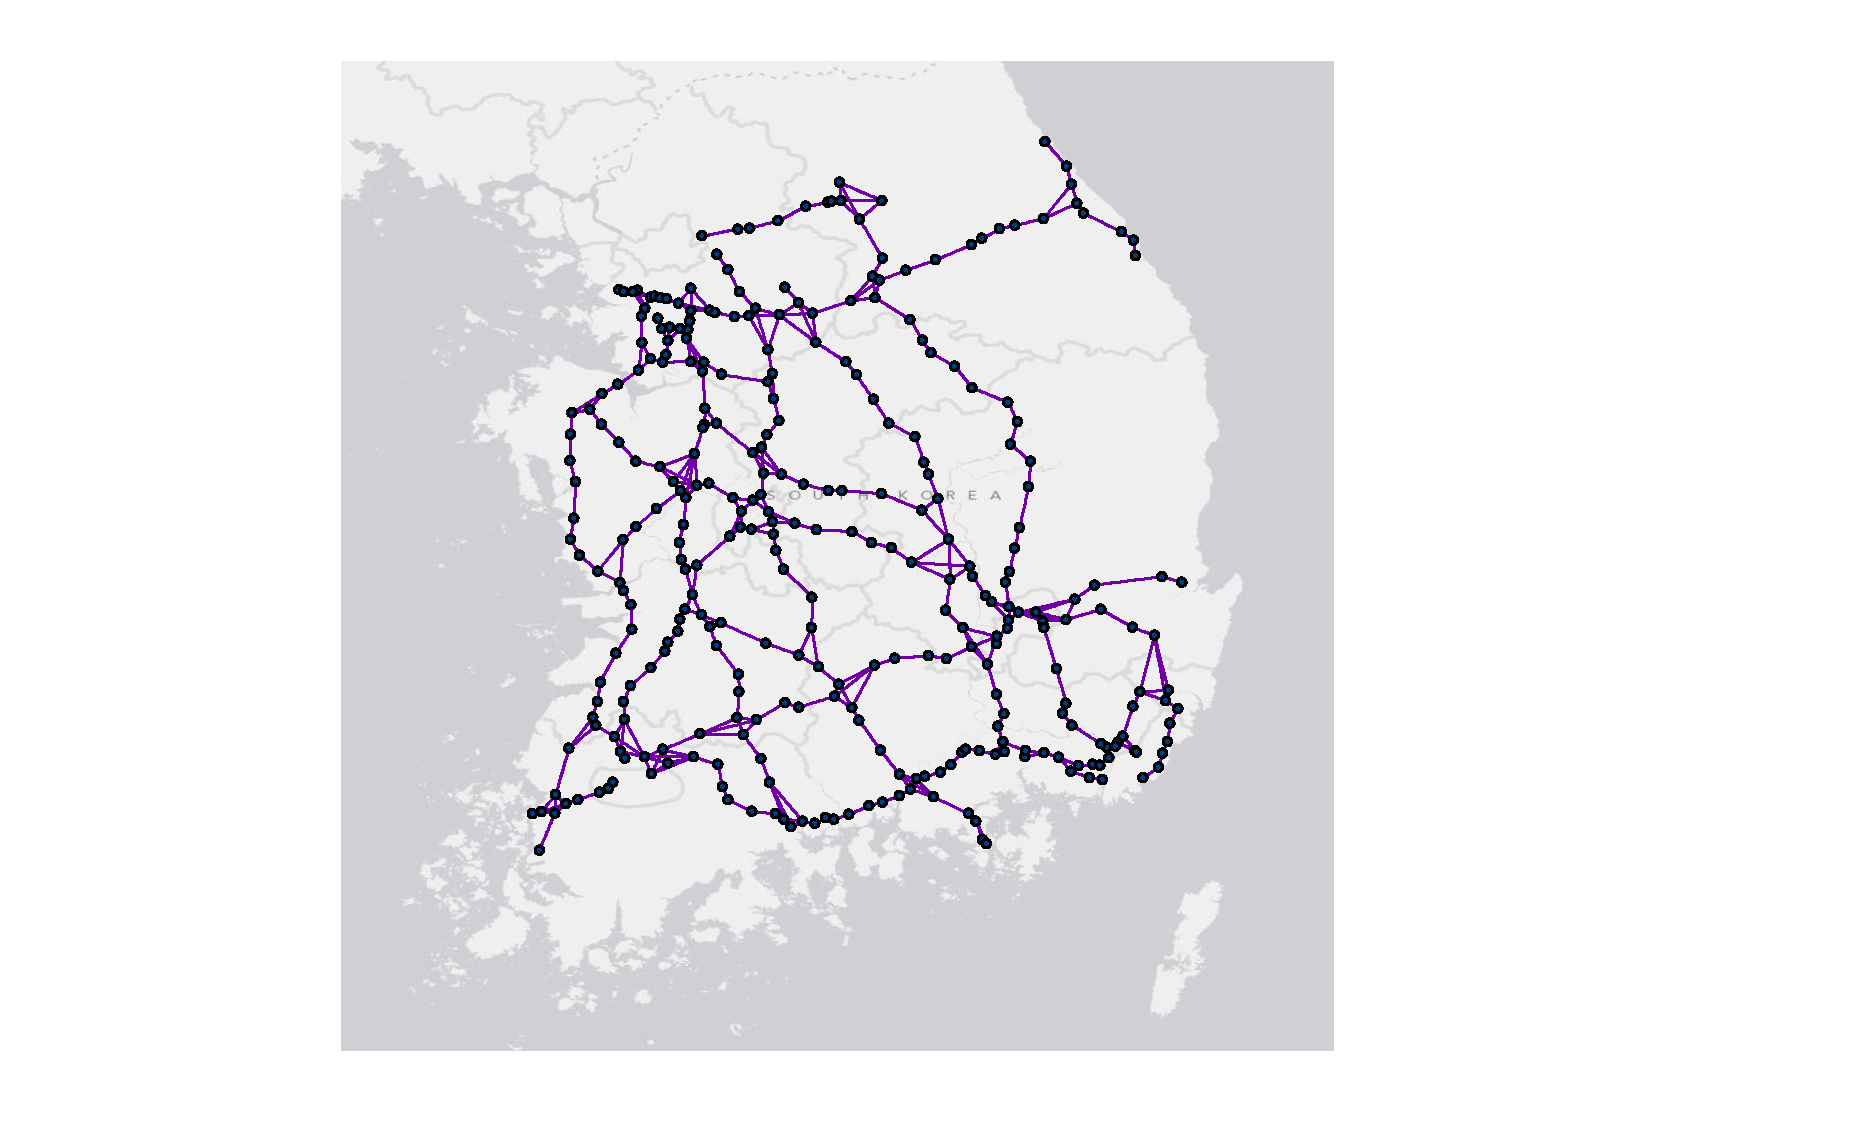
\includegraphics[width=2in]{map}
\caption{Vector-based PDF}
\label{fig:map-pdf}
\end{subfigure}
%
\begin{subfigure}[b]{0.4\textwidth}
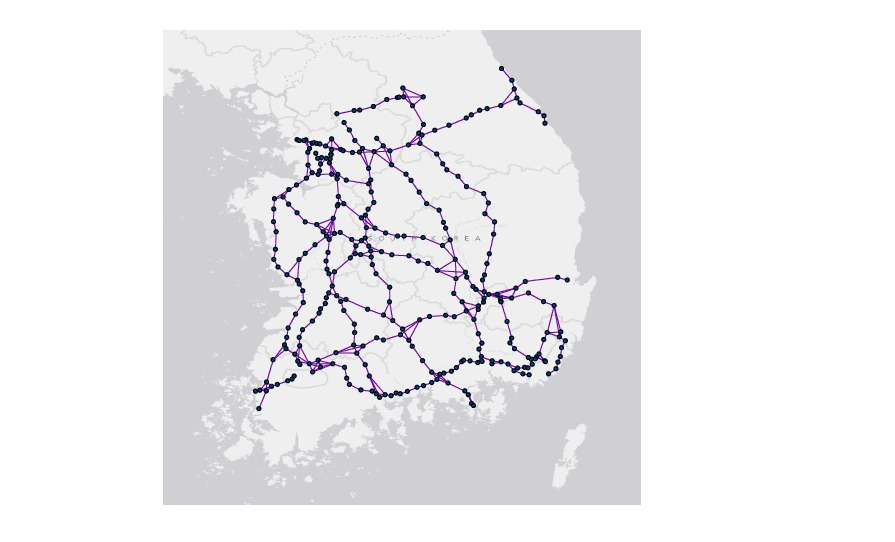
\includegraphics[width=4in]{map-jpg}
\caption{PDF converted from JPG}
\label{fig:map-jpg}
\end{subfigure}
\caption{Figures side by side using \texttt{subfigure}. Zoom in to see the differences.}
\label{fig:side-by-side}
\end{figure}







% Bibliography
\bibliographystyle{ormsv080-ck}		% Bibliography style. Journals/conferences may require something different
\bibliography{sample_ref}			% Your .bib filename goes here


% If you need appendices.
\newpage
\renewcommand{\appendixpagename}{Appendix}

\appendix
\appendixpage

This is appendix.

\section{Proofs} \label{appendix:proofs}

You may want to collect proofs for theorems here. This is Appendix \ref{appendix:proofs}.

\section{Data} \label{appendix:data}

Or maybe some data. This is Appendix \ref{appendix:data}.

\end{document}







%

